\documentclass[10pt]{article}

% RLJ/RLC 2026 submission mode. Use [accepted] or [preprint] only for those
% versions of the paper.
\usepackage[preprint]{rlj}

\usepackage{amssymb}
\usepackage{array}
\usepackage{float}
\usepackage{graphicx}
\usepackage{placeins}
\usepackage{tikz}
\usepackage{xurl}
\usetikzlibrary{arrows.meta,calc,decorations.pathreplacing,fit,positioning}

\tikzset{
  conceptfig/.style={>=Stealth,
    every node/.style={font=\small,align=center}},
  setnode/.style={draw,inner sep=5pt},
  procnode/.style={draw,rounded corners=2pt,fill=black!8,inner ysep=4pt,
    inner xsep=6pt,minimum width=2.3cm},
  note/.style={font=\scriptsize},
  substep/.style={circle,fill,inner sep=1.4pt},
  fragment/.style={draw=black!60,dashed,rounded corners=2pt,inner sep=4pt},
}

\graphicspath{{figures/}}

\newcommand{\papergrid}[2][0.18]{%
  \begin{tikzpicture}[x=#1cm,y=-#1cm,baseline=(current bounding box.center)]
    \fill[white] (0,0) rectangle (10,10);
    #2
    \draw[step=1,gray!35,line width=0.18pt] (0,0) grid (10,10);
    \draw[gray!55,line width=0.35pt] (0,0) rectangle (10,10);
  \end{tikzpicture}%
}

\newcommand{\papervertical}{%
  \foreach \r in {0,...,9}{\fill[black] (5,\r) rectangle +(1,1);}%
}

\newcommand{\paperdiagonal}{%
  \foreach \i in {0,...,9}{\fill[black] (\i,\i) rectangle +(1,1);}%
}

\newcommand{\papersquare}{%
  \foreach \i in {0,...,9}{%
    \fill[black] (\i,0) rectangle +(1,1);
    \fill[black] (\i,9) rectangle +(1,1);
    \fill[black] (0,\i) rectangle +(1,1);
    \fill[black] (9,\i) rectangle +(1,1);%
  }%
}

\newcommand{\papergridlabel}[3][0.18]{%
  \begin{tabular}{@{}c@{}}
    \papergrid[#1]{#2}\\[-0.15em]
    {\scriptsize #3}
  \end{tabular}%
}

\title{On the Value of Abstractions: Abstraction Selection in Bounded Program Synthesis}
\setrunningtitle{Abstraction Selection in Bounded Program Synthesis}
\hypersetup{
  pdftitle={On the Value of Abstractions: Abstraction Selection in Bounded Program Synthesis},
  pdfauthor={Adam Cuculich}
}

\author{Adam Cuculich}
\emails{adam@cuculich.me}
\affiliations{}

\keywords{abstraction selection, bounded program synthesis, library learning, search cost minimization}

\summary{Reusable abstractions can shorten programs in program synthesis. Some
do not improve bounded search. We compare two selection procedures on a
synthetic grid benchmark.
With ten abstractions, both procedures solved more problems than primitive-only
search. Search cost minimization solved 4.08 more test problems per 100 than
compression scoring the same selection problems (95 percent CI 2.46 to 5.71).
This comparison includes what each procedure scores and whether it includes
unsolved problems. At 30,000 attempts, observed mean performance was highest at
11 abstractions. With 20 abstractions, both procedures performed worse than
primitives. In this
benchmark, abstraction value depended on selection method, library size, and
search budget.}

\contribution{
Search cost minimization selects the abstractions that decrease capped search
cost most on a separate problem set.
}{
Compression selects the abstractions that shorten known solutions most.
}

\contribution{
With ten abstractions, both procedures solved more test problems than
primitive-only search. Search cost minimization solved 4.08 more test problems
per 100 than compression scoring the same selection problems.
}{
Primitive-only problems provide the same candidate set for both procedures. Separate test
problems measure held-out performance.
}

\contribution{
At 30,000 attempts, observed mean performance was highest at 11 abstractions.
With 20 abstractions, both procedures performed worse than primitives alone.
}{
For these fixed one- and two-abstraction libraries, a larger budget reversed
the decrease.
}

\begin{document}

\maketitle

\begin{abstract}
Library learning allows a computational solver to use its experience solving problems to add abstractions to its library that aid in future problem solving. How it chooses those abstractions, however, affects its performance on unseen test problems. Additionally, the value of each abstraction a solver adds to its library is contextually dependent on factors like: its search process, search budgets, and library size. In this paper, we explore two different approaches for selecting abstractions and test the performance of the resulting libraries they construct. Namely, we compare \textbf{compression}--which chooses abstractions that compress the size of a set of previously-found past solution programs by minimizing the number of subprograms across the entire set--against \textbf{search cost minimization}--which chooses abstractions that minimize solution search cost on a new distinct problem set. Both selection procedures choose abstractions from the same set of subprogram candidates, created by initially finding solution programs using only primitive substates and operations that are permitted by a starter domain specific language (DSL). We used Pattern Builder for this study, which presents a solver with a pattern on a 10x10 pixel grid and tasks it to build a program using its library that constructs that pattern. Asking how a solver should optimally add subprograms to its library is worthwhile not only because it can improve held-out problem-solving performance but also because the procedures by which abstractions are chosen differ in computational cost: any increased performance should justify the computational cost required to achieve it. This paper also explores how library size affects solver performance under both abstraction selection procedures under a fixed search budget--and how a search budget interacts with library size and test performance. Each subprogram added to a library increases the number of possible shallow-depth programs a solver must search through, which can exhaust its search budget. While abstractions themselves reduce search by not requiring solvers to reconstruct their subprograms, it's possible that this search reduction is only used deeper into a program trajectory. Such cases may exhaust a search budget before a solution program is found, highlighting a tradeoff between library size and search cost.

In this study, we found that with 10 abstractions, both selection procedures outperformed the primitive-only DSL. When both abstraction selection methods used the same set of problems, search cost minimization solved 4.08 more test problems out of 100 than compression. At 30,000 program attempts, mean performance peaked at 11 abstractions but then fell sharply, ultimately underperforming the primitive-only DSL at 20 added abstractions. Interestingly, both selection procedures' library performance dropped sharply from library size 1 to 2 abstractions. We determined that this performance drop was caused by the 30,000 program search budget: after holding the libraries constant and increasing allowed search, all of the unsolved problems that constituted the performance reduction were recovered. These findings strongly support the view the value of a library abstraction depends on the context in which it's used and the constraints a solver is subject to.
\end{abstract}

\section{Introduction}

Pattern Builder provides the program-synthesis task in this paper. Each
problem presents a solver with a pattern on a binary $10\times10$ pixel grid,
and the solver must build a program that constructs that pattern. It starts
with no input grid and combines six primitive grids with fixed operations
until a program's output matches the target.
Figure~\ref{fig:problem-solution} shows one target and one program that builds
it. The operation \texttt{add} returns the union of two grids.
\begin{figure}[H]
  \centering
  \begin{tabular}{@{}c@{\hspace{0.03\linewidth}}c@{}}
    \parbox{0.25\linewidth}{\centering\textbf{Target}}
    &
    \parbox{0.70\linewidth}{\centering\textbf{One valid solution}}
    \\[0.5em]
    \begin{minipage}[t]{0.25\linewidth}
      \vspace{0pt}
      \centering
      \papergridlabel[0.20]{\papersquare\papervertical\paperdiagonal}{target grid}
    \end{minipage}
    &
    \begin{minipage}[t]{0.70\linewidth}
      \vspace{0pt}
      \centering
      \papergridlabel[0.125]{\papervertical}{\texttt{line\_vertical}}
      \hspace{0.25em}$+$\hspace{0.25em}
      \papergridlabel[0.125]{\papersquare}{\texttt{square}}
      \hspace{0.25em}$+$\hspace{0.25em}
      \papergridlabel[0.125]{\paperdiagonal}{\texttt{diagonal}}
      \hspace{0.25em}$=$\hspace{0.25em}
      \papergridlabel[0.125]{\papersquare\papervertical\paperdiagonal}{output}
      \\[0.7em]
      \texttt{add(add(line\_vertical, square), diagonal)}
    \end{minipage}
  \end{tabular}
  \caption{A grid target and one expression that reproduces it.}
  \label{fig:problem-solution}
\end{figure}

We call each target-grid task a problem $T_i$ and write its problem state as
$S_i^{\mathrm{problem}}$. A solution program $P_i$ transforms that problem
state into a solution state $S_i^{\mathrm{solution}}$ that matches the target
grid:
\[
  S_i^{\mathrm{problem}} \xrightarrow{\;P_i\;} S_i^{\mathrm{solution}}.
\]
A solution program is a composite function, possibly nested, and its parts are
\emph{subprograms}. The intermediate grids a program produces while it
executes are \emph{substates}. Operations transform substates in two ways. A
unary operation $f_u$ applies directly to one substate and produces another,
while a binary operation $f_b$ combines two substates and produces another:
\[
  S_1 \xrightarrow{\;f_u\;} S_2,
  \qquad
  (S_1,S_2) \xrightarrow{\;f_b\;} S_3.
\]
Figure~\ref{fig:program-structure} shows how substates, operations, and
subprograms compose into a solution program.

\begin{figure}[H]
  \centering
  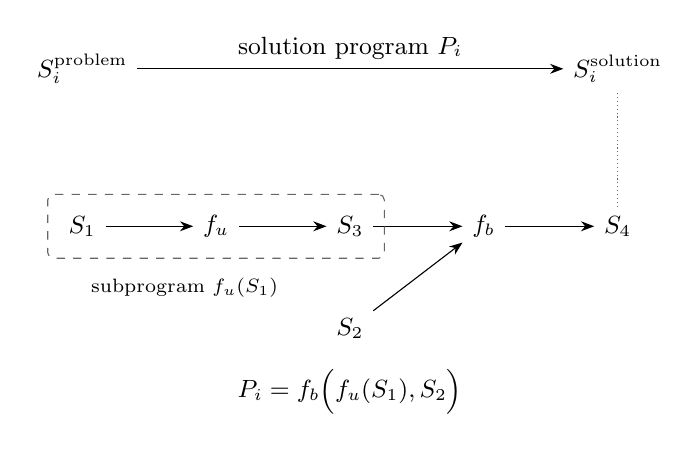
\begin{tikzpicture}[conceptfig]
    \node (problem) at (0,0) {$S_i^{\mathrm{problem}}$};
    \node (solution) at (6.8,0) {$S_i^{\mathrm{solution}}$};
    \draw[->] (problem) -- node[midway,above] {solution program $P_i$}
      (solution);

    \node (sone) at (0,-2.0) {$S_1$};
    \node (unary) at (1.7,-2.0) {$f_u$};
    \node (sthree) at (3.4,-2.0) {$S_3$};
    \node (stwo) at (3.4,-3.3) {$S_2$};
    \node (binary) at (5.1,-2.0) {$f_b$};
    \node (sfour) at (6.8,-2.0) {$S_4$};
    \draw[->] (sone) -- (unary);
    \draw[->] (unary) -- (sthree);
    \draw[->] (sthree) -- (binary);
    \draw[->] (stwo) -- (binary);
    \draw[->] (binary) -- (sfour);
    \draw[densely dotted,black!60] (sfour) -- (solution);

    \node[fragment,fit=(sone)(unary)(sthree)] (sub) {};
    \node[note,below=0.12cm of sub,xshift=-0.4cm] {subprogram $f_u(S_1)$};
    \node at (3.4,-4.1) {$P_i=f_b\bigl(f_u(S_1),S_2\bigr)$};
  \end{tikzpicture}
  \caption{One solution program from the inside. The program $P_i$ maps the
  problem state to the solution state. Within it, the unary operation $f_u$
  transforms substate $S_1$ into substate $S_3$, and the binary operation
  $f_b$ combines $S_3$ with $S_2$ to produce $S_4$, which is the solution
  state. The fragment $f_u(S_1)$ is one subprogram of $P_i$.}
  \label{fig:program-structure}
\end{figure}

The solver does not know which program will construct the target, so it
searches. At each substate, it can apply a unary operation or combine that
substate with another through a binary operation, and it works through these
possible operations and transitions until a program's output matches the
target. The solver first solves problems with primitives only. We call those
problems the primitive-only problem set, $T_{\mathrm{prim}}$; it
exists to give the solver experience before any abstractions are available.
The successful programs the solver finds on it form the primitive-only
solution program set,
\[
  P_{\mathrm{prim}}
  = \{P_{1,\mathrm{prim}},\ldots,P_{n,\mathrm{prim}}\},
\]
where each $P_{i,\mathrm{prim}}$ solves its problem $T_i$. This set is the
solver's empirical experience, and it is the only place we look for
abstractions: every subprogram found within a primitive-only solution program
is an \emph{abstraction candidate}. Together, the candidates form the set
\[
  A_{\mathrm{candidates}}
  = \bigcup_{P\in P_{\mathrm{prim}}}\operatorname{subprograms}(P).
\]
Figure~\ref{fig:solver-experience} traces this path from problems to solution
programs to candidates.

\begin{figure}[H]
  \centering
  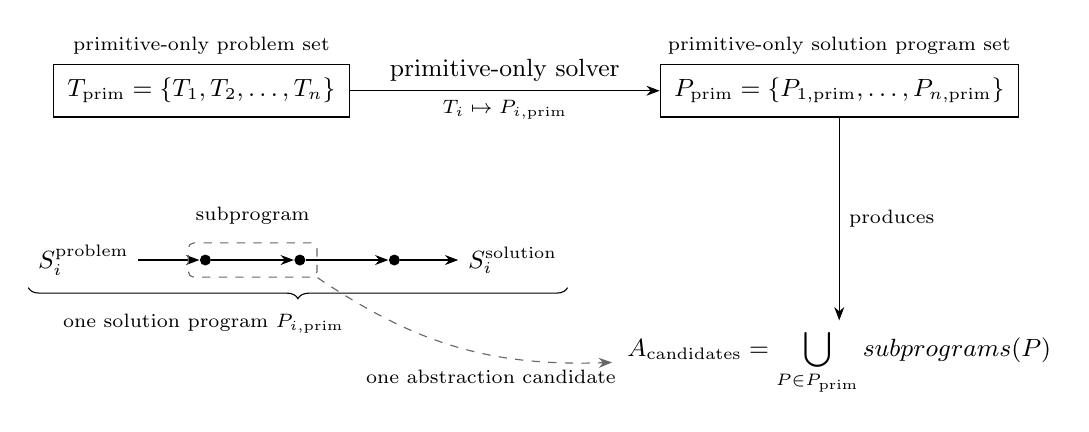
\begin{tikzpicture}[conceptfig]
    \node[setnode,label={[note]above:primitive-only problem set}]
      (tprim) at (0,0)
      {$T_{\mathrm{prim}}=\{T_1,T_2,\ldots,T_n\}$};
    \node[setnode,label={[note]above:primitive-only solution program set}]
      (pprim) at (8.1,0)
      {$P_{\mathrm{prim}}
        =\{P_{1,\mathrm{prim}},\ldots,P_{n,\mathrm{prim}}\}$};
    \draw[->] (tprim) -- node[midway,above] {primitive-only solver}
      node[midway,below,note] {$T_i\mapsto P_{i,\mathrm{prim}}$} (pprim);

    \node (zin) at (-1.5,-2.15) {$S_i^{\mathrm{problem}}$};
    \node[substep] (zda) at (0.05,-2.15) {};
    \node[substep] (zdb) at (1.25,-2.15) {};
    \node[substep] (zdc) at (2.45,-2.15) {};
    \node (zout) at (3.95,-2.15) {$S_i^{\mathrm{solution}}$};
    \draw[->] (zin) -- (zda);
    \draw[->] (zda) -- (zdb);
    \draw[->] (zdb) -- (zdc);
    \draw[->] (zdc) -- (zout);
    \draw[decorate,decoration={brace,mirror,amplitude=4pt}]
      (-2.2,-2.5) -- (4.65,-2.5)
      node[midway,below=6pt,note,xshift=-1.2cm]
      {one solution program $P_{i,\mathrm{prim}}$};
    \node[fragment,fit=(zda)(zdb)] (zfrag) {};
    \node[note,above=0.1cm of zfrag] {subprogram};

    \node (acand) at (8.1,-3.45)
      {$A_{\mathrm{candidates}}
        =\displaystyle\bigcup_{P\in P_{\mathrm{prim}}}
        \operatorname{subprograms}(P)$};
    \draw[->] (pprim) -- node[midway,right,note] {produces} (acand);
    \draw[->,dashed,black!60] (zfrag.south east) to[bend right=18]
      node[pos=0.62,below=2pt,note,black] {one abstraction candidate}
      ([xshift=-2pt]acand.west);
  \end{tikzpicture}
  \caption{From solver experience to abstraction candidates. The
  primitive-only solver solves each problem $T_i$ in
  $T_{\mathrm{prim}}$, and the solution programs it finds form
  $P_{\mathrm{prim}}$, the solver's experience. Every subprogram
  found within those programs, such as the marked fragment of
  $P_{i,\mathrm{prim}}$, enters the abstraction candidate set
  $A_{\mathrm{candidates}}$.}
  \label{fig:solver-experience}
\end{figure}

An \emph{abstraction} is a selected subprogram stored as one item in the
solver's library. During search, the solver can use a stored abstraction
directly, without reconstructing its internal subprograms. A selector decides
which candidates earn that place: it chooses a subset $A^{*}_q$ of
$A_{\mathrm{candidates}}$ and adds it to the primitive library
$L_{\mathrm{prim}}$, producing the library
\[
  L_q = L_{\mathrm{prim}} \cup A^{*}_q,
\]
where $q$ names the selector.
This leads to the fundamental question of the paper: how should a solver
select abstractions from its experience if its goal is maximum
problem-solving performance on an unseen test problem set?

We compare two selectors that answer this question differently.
\textbf{Compression} chooses the abstractions that minimize the number of
subprograms needed to represent the primitive-only solution programs, so it
works entirely from solutions the solver has already found. \textbf{Search
cost minimization} instead measures candidates in use: it chooses the
abstractions that empirically minimize search cost on the \emph{Search Cost
Minimization Problem Set}, $T_{\mathrm{SCM}}$, a new problem set
that exists only to supply that measurement. Selecting from the same
candidates, the two selectors produce the selected abstraction sets
$A^{*}_{\mathrm{compression}}$ and
$A^{*}_{\mathrm{search\ cost}}$, and with them the libraries
$L_{\mathrm{compression}}$ and $L_{\mathrm{search\ cost}}$. To measure which
library is better, we reserve the unseen test problem set,
$T_{\mathrm{test}}$: a set of problems no selector ever sees, so
performance on it shows how well the selected abstractions generalize. The
same solver attempts the same test problems with each library.
Figure~\ref{fig:abstraction-selection} shows this comparison.

\begin{figure}[H]
  \centering
  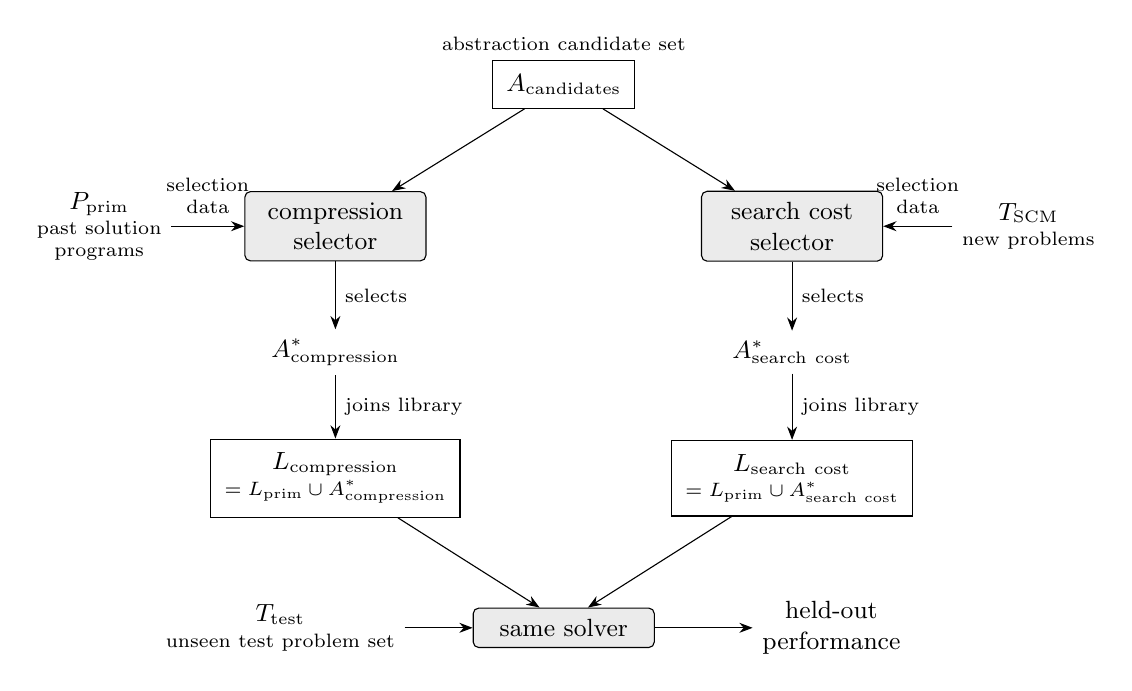
\begin{tikzpicture}[conceptfig]
    \node[setnode,label={[note]above:abstraction candidate set}]
      (acand) at (0,0) {$A_{\mathrm{candidates}}$};
    \node[procnode] (comp) at (-2.9,-1.8) {compression\\selector};
    \node[procnode] (scm) at (2.9,-1.8) {search cost\\selector};
    \draw[->] (acand) -- (comp);
    \draw[->] (acand) -- (scm);

    \node (pprim) at (-5.9,-1.8)
      {$P_{\mathrm{prim}}$\\[-0.2em]
       {\scriptsize past solution}\\[-0.35em]{\scriptsize programs}};
    \node (tscm) at (5.9,-1.8)
      {$T_{\mathrm{SCM}}$\\[-0.2em]
       {\scriptsize new problems}};
    \draw[->] (pprim) -- node[midway,above=1pt,note] {selection\\data} (comp);
    \draw[->] (tscm) -- node[midway,above=1pt,note] {selection\\data} (scm);

    \node (astarc) at (-2.9,-3.4) {$A^{*}_{\mathrm{compression}}$};
    \node (astars) at (2.9,-3.4) {$A^{*}_{\mathrm{search\ cost}}$};
    \draw[->] (comp) -- node[midway,right,note] {selects} (astarc);
    \draw[->] (scm) -- node[midway,right,note] {selects} (astars);

    \node[setnode] (lcomp) at (-2.9,-5.0)
      {$L_{\mathrm{compression}}$\\[-0.2em]
       {\scriptsize $=L_{\mathrm{prim}}\cup A^{*}_{\mathrm{compression}}$}};
    \node[setnode] (lscm) at (2.9,-5.0)
      {$L_{\mathrm{search\ cost}}$\\[-0.2em]
       {\scriptsize $=L_{\mathrm{prim}}\cup A^{*}_{\mathrm{search\ cost}}$}};
    \draw[->] (astarc) -- node[midway,right,note] {joins library} (lcomp);
    \draw[->] (astars) -- node[midway,right,note] {joins library} (lscm);

    \node[procnode] (solver) at (0,-6.9) {same solver};
    \draw[->] (lcomp) -- (solver.140);
    \draw[->] (lscm) -- (solver.40);
    \node (ttest) at (-3.6,-6.9)
      {$T_{\mathrm{test}}$\\[-0.2em]
       {\scriptsize unseen test problem set}};
    \draw[->] (ttest) -- (solver);
    \node (perf) at (3.4,-6.9) {held-out\\performance};
    \draw[->] (solver) -- (perf);
  \end{tikzpicture}
  \caption{Two selection paths from one candidate set. Both selectors choose
  from $A_{\mathrm{candidates}}$, but compression scores candidates
  against the primitive-only solution programs, while search cost
  minimization scores them by empirical search cost on the Search Cost
  Minimization Problem Set. Each selected set joins the primitive library,
  and the same solver then attempts the same unseen test problems with each
  resulting library.}
  \label{fig:abstraction-selection}
\end{figure}

For example, the union of \texttt{line\_vertical} and \texttt{square} in
Figure~\ref{fig:problem-solution} is one abstraction candidate. Storing it can
shorten a later program, yet it also becomes one more item the solver must
consider at every substate during search. Under a fixed search budget, a
larger library can spend its attempts on shallow programs before the solver
ever reaches the deeper program where an abstraction pays off. An
abstraction's value therefore depends on library size, the search process,
and the search budget.

Selection itself has a computational cost, and that cost differs between
the two selectors.
Compression reuses solution programs the solver already has, while search
cost minimization requires the solver to work through the Search Cost
Minimization Problem Set before it selects anything. This gap is part of why
the comparison is worthwhile: any increase in held-out performance should
justify the computational cost required to achieve it.

Experiment I compares the selectors while changing the similarity between the
selection problems and the unseen test problems, which reduces shared motifs
as a source of performance. Experiment II changes the number of selected
abstractions under a fixed search budget. Experiment III holds the libraries
fixed and changes the search budget. Together, the three experiments test how
selection objective, library size, and available search shape the value of an
abstraction.
\section{Related Work}

Library learning adds reusable program components to a solver's library so
that later synthesis becomes easier, and many systems choose those components
by compressing known solution programs. DreamCoder learns a function library
together with a neural search policy \citep{ellis2021dreamcoder}. Stitch finds
the functions that minimize the cost of a rewritten program corpus
\citep{bowers2023stitch}. A recent study used Pattern Builder to examine which
helper programs people choose as task structure changes
\citep{hernandezcano2026prospective}; their choices were consistent with
compression of expected future solutions. Our study instead measures how
automated abstraction selection changes bounded search.

Iba described the search tradeoff that motivates this measurement: macros
shorten solution paths and increase the search branching factor
\citep{iba1989macro}. AbstractBeam later added Stitch abstractions to guided
bottom-up synthesis and improved performance on related tasks, but a
distribution shift removed the benefit, and unused abstractions could enlarge
the language \citep{zenkner2024abstractbeam}. AMaze provides the closest
technical comparison: it modifies a domain-specific language (DSL) using
predicted synthesis time,
estimated from the enumeration rank of solver-specific program fragments, and
its whole-program compression baseline slowed two of four synthesizers
\citep{ye2026amaze}. Our work measures capped search cost directly, with exact
enumeration over a fixed candidate set within each seed. We vary library
size, change only the search budget for fixed libraries, and measure the work
each selection procedure spends to select its library. These controls test
how selection objective, library size, and search budget jointly determine an
abstraction's value.
\section{Methodology}

\subsection{Experiment Overview}

We test how abstraction selection affects bounded-search performance, and
later experiments change library size and search budget. Experiment I
compares four selection procedures: three compression variants that differ in
the solution programs they score, and search cost minimization. Each
procedure selects from the same abstraction candidate set, and we then test
each selected library on the same held-out problems.

The three problem sets of the introduction carry the design. The
primitive-only problem set $T_{\mathrm{prim}}$ contains 100
problems; it creates the abstraction candidate set and supplies the solution
programs that two compression variants score. The Search Cost Minimization
Problem Set $T_{\mathrm{SCM}}$ contains 25 new problems; search
cost minimization scores search cost on it directly, and one compression
variant scores solution programs acquired for it. The unseen test problem set
$T_{\mathrm{test}}$ contains 100 problems that no procedure sees;
we reserve it for held-out evaluation.
We repeat the experiment across 30 random problem worlds. Each seed creates
one world with 12 hidden motifs, the grids from which the generator builds
every target, and one primitive-only problem set shared by
six primary conditions, each with a separate $T_{\mathrm{SCM}}$ and
$T_{\mathrm{test}}$.
Table~\ref{tab:problem-sets} gives the size and purpose of each problem set.

\begin{table}[H]
  \centering
  \small
  \caption{Problem sets and their use.}
  \label{tab:problem-sets}
  \vspace{0.7em}
  \begin{tabular*}{0.95\linewidth}{@{\extracolsep{\fill}}>{\raggedright\arraybackslash}p{0.30\linewidth}rp{0.55\linewidth}@{}}
    \hline
    \textbf{Problem Set} & \textbf{Size} & \textbf{Purpose} \\
    \hline
    \noalign{\vskip 0.25em}
    Primitive-only problem set ($T_{\mathrm{prim}}$) & 100 & Creates the abstraction candidate set and supplies solution programs for compression. \\
    Search Cost Minimization Problem Set ($T_{\mathrm{SCM}}$) & 25 & Supplies the selection data for search cost minimization and one compression variant. \\
    Unseen test problem set ($T_{\mathrm{test}}$) & 100 & Measures each selected library on held-out problems. \\
    \hline
  \end{tabular*}
\end{table}

Each seed has one abstraction candidate set of 50 candidates, and every
selection procedure selects from it.
Table~\ref{tab:selection-procedures} defines the four selection procedures
and the labels that later equations use. The three compression variants score
different solution program sets: all of $P_{\mathrm{prim}}$, the
subset $P_{\mathrm{prim,25}}$ acquired for a fixed 25-problem
subset $T_{\mathrm{prim,25}}\subset T_{\mathrm{prim}}$, or
the set $P_{\mathrm{SCM}}$ of solution programs the solver acquires
for the Search Cost Minimization Problem Set:
\[
  T_{\mathrm{SCM}}
  \xrightarrow{\;\text{solver}\;}
  P_{\mathrm{SCM}}.
\]
The fourth procedure, search cost minimization, scores search cost on
$T_{\mathrm{SCM}}$ directly.

\begin{table}[!htbp]
  \centering
  \footnotesize
  \caption{Four selection procedures in Experiment I.}
  \label{tab:selection-procedures}
  \vspace{0.7em}
  \setlength{\tabcolsep}{4pt}
  \renewcommand{\arraystretch}{1.12}
  \begin{tabular*}{0.95\linewidth}{@{\extracolsep{\fill}}>{\raggedright\arraybackslash}p{0.115\linewidth}>{\raggedright\arraybackslash}p{0.235\linewidth}>{\raggedright\arraybackslash}p{0.135\linewidth}>{\raggedright\arraybackslash}p{0.20\linewidth}>{\raggedright\arraybackslash}p{0.183\linewidth}@{}}
    \hline
    \textbf{Label} & \textbf{Selection procedure} & \textbf{Selection data} & \textbf{Search during selection} & \textbf{Score} \\
    \hline
    \noalign{\vskip 0.25em}
    \mbox{$\mathrm{comp\text{-}100}$} & Compression on all primitive-only solution programs & $P_{\mathrm{prim}}$ (100 problems) & Acquire solutions; 30,000 attempts per problem & Remaining operations in acquired solutions \\
    \mbox{$\mathrm{comp\text{-}25}$} & Compression on a 25-problem primitive-only subset & $P_{\mathrm{prim,25}}$ (25 problems) & Acquire solutions; 30,000 attempts per problem & Remaining operations in acquired solutions \\
    \mbox{$\mathrm{comp\text{-}SCM}$} & Compression on solution programs acquired for $T_{\mathrm{SCM}}$ & $P_{\mathrm{SCM}}$ (25 problems) & Acquire solutions; 90,000 attempts per problem & Remaining operations in acquired solutions \\
    \mbox{$\mathrm{scm}$} & Search cost minimization on $T_{\mathrm{SCM}}$ & $T_{\mathrm{SCM}}$ (25 problems) & Score each trial library; 30,000 attempts & Mean capped search cost for all 25 problems \\
    \hline
  \end{tabular*}
\end{table}

Each compression variant runs a separate target-directed search for each
scoring problem, keeps the first solution found, and omits unsolved problems.
Compression can only score problems that produced a solution, so compression
on $P_{\mathrm{SCM}}$ uses a larger 90,000-attempt acquisition budget on
$T_{\mathrm{SCM}}$.
Search cost minimization runs one size-ordered search for each trial library,
whose output record scores all 25 problems of $T_{\mathrm{SCM}}$,
and an unreached target receives the maximum cost of 30,000. Hidden generator
programs are never selector inputs. A fixed seeded shuffle selects the 25
problems of $T_{\mathrm{prim,25}}$, and all six conditions within a
seed use the same subset. Across the 180 primary Experiment I cells,
acquisition produced solutions for a mean of 62.70 of the 100 problems in
$T_{\mathrm{prim}}$, 16.33 of the 25 in
$T_{\mathrm{prim,25}}$, and 16.59 of the 25 in
$T_{\mathrm{SCM}}$.

In Experiment I, each procedure selects ten abstractions. We evaluate every
selected library on the same 100 test problems with a 30,000-attempt limit.
The primary comparison between search cost minimization and compression on
$P_{\mathrm{SCM}}$ uses the same 25 problems of
$T_{\mathrm{SCM}}$. Search cost minimization scores all 25
outcomes, whereas compression on $P_{\mathrm{SCM}}$ scores only
acquired solution programs and omits a mean of 8.41 unsolved problems.
The comparison holds the candidate set, test problems, library size, and test
budget constant, so it compares complete procedures that differ in what they
score and whether they include unsolved problems.

\subsection{Synthesis and Bounded Search}

Each problem $T_i$ presents one binary target grid, the grid its solution
state $S_i^{\mathrm{solution}}$ must match. The primitive library
$L_{\mathrm{prim}}$ contains six grids: blank, horizontal line, vertical
line, diagonal, square, and triangle. Let $L$ denote the current ordered
library. A program is a library item or an operation applied to one or two
programs. The unary operations form the set $F_u$, with
$f_u\in F_u$: invert, a left-to-right flip, a top-to-bottom flip,
and diagonal reflection. The diagonal grid runs from the upper-left corner to
the lower-right corner. Invert changes each black cell to white and each
white cell to black. The binary operations form the set $F_b$, with
$f_b\in F_b$: \texttt{add} (union), \texttt{subtract} (set
difference), and \texttt{overlap} (intersection). Program $P$ produces grid
$\operatorname{eval}(P)$ and solves $T_i$ when $\operatorname{eval}(P)$
equals the target grid of $T_i$.
Program size is the number of operation applications. A primitive or stored
abstraction has size zero. Let $B$ be the maximum number of candidate programs
that the solver can try. The deterministic bottom-up solver tries programs in
order of increasing size. It stops after $B$ attempts or after it has tried all
programs with seven or fewer operation applications. The solver keeps the first
program for each distinct output grid. The implementation fixes the order of
operations, child-program sizes, and commutative arguments. Each generated
program counts as one search attempt. If it produces an output grid that the
solver has already seen, the solver discards it after counting the attempt.
For search cost minimization scoring and final evaluation, one size-ordered
search records all outputs for a library and the first attempt that produced
each target. Compression uses separate target-directed searches
to acquire solution programs.

Search cost is a function of a problem, a library, and a budget:
\[
  (T_i, L, B) \xrightarrow{\;\text{solver}\;} N_B(T_i, L).
\]
$N_B$ measures how many attempts the solver needs to reach the target grid of
$T_i$, capped at the budget:
\begin{equation}
  N_B(T_i,L)=
  \begin{cases}
    n, & \text{if the target grid of $T_i$ first appears at attempt $n\leq B$},\\
    B, & \text{if the solver does not reach it within the budget}.
  \end{cases}
\end{equation}
Unless stated otherwise, $B=30{,}000$. We use the number of held-out test
targets reached among 100 as our primary outcome.

\subsection{The Abstraction Candidate Set}

The introduction builds the abstraction candidate set through the chain
\[
  T_{\mathrm{prim}}
  \xrightarrow{\;\text{primitive-only solver}\;}
  P_{\mathrm{prim}}
  \xrightarrow{\;\operatorname{subprograms}(\cdot)\;}
  A_{\mathrm{candidates}}.
\]
The full set of subprograms is too large to score repeatedly, so the
experiment bounds $A_{\mathrm{candidates}}$ to 50 candidates in two
stages. Each candidate is a subprogram. If selected, the solver stores the
candidate's output grid as a size-zero library item and can then use that
grid without rebuilding the subprogram from primitives. The candidate set
therefore defines the available library modifications, while the selection
procedures determine which modifications are made.

The first stage collects reached grids. The primitive-only solver uses the
standard 30,000-attempt budget and records the first program found for each
distinct output grid. We exclude the blank grid and the six primitive grids
because the library already contains them. We keep grids whose first programs
have one to four operations, which yields nontrivial candidates while
limiting the initial pool to small subprograms.

The second stage keeps candidates with observed potential for reuse. We apply
the same one-step test to every target grid of $T_{\mathrm{prim}}$
separately. A candidate supports a target if one additional invert or
reflection can produce that target from the candidate's grid, or if one add
or subtract involving another reached grid can do so. The support count is
the number of distinct targets that satisfy this test. We retain only
candidates with a support count of at least two, the smallest count that
indicates potential reuse across problems.

We rank the retained candidates by decreasing support count, then break ties
by the attempt at which the primitive-only solver first reached the grid and
by program string. The top 50 candidates form the experiment's
$A_{\mathrm{candidates}}$. This cap keeps repeated candidate
evaluation tractable, while the fixed ranking and tie rules make construction
deterministic. Construction uses no problems from
$T_{\mathrm{SCM}}$ or $T_{\mathrm{test}}$, and every
selection procedure within a problem world receives the same fixed candidate
set. The next subsection describes how each procedure selects abstractions
from $A_{\mathrm{candidates}}$, one at a time.

\subsection{Selection Procedures}

Each selection procedure builds its library one abstraction at a time. A
selector takes the candidate set, its own selection data, and a target
library size $K$, and returns the selected abstraction set:
\begin{gather*}
  \operatorname{Select}_{\mathrm{compression}}
    \bigl(A_{\mathrm{candidates}},\,P_{\mathrm{score}},\,K\bigr)
    \longrightarrow A^{*}_{K},\\
  \operatorname{Select}_{\mathrm{search\ cost}}
    \bigl(A_{\mathrm{candidates}},\,T_{\mathrm{SCM}},\,B,\,K\bigr)
    \longrightarrow A^{*}_{K}.
\end{gather*}
Here $P_{\mathrm{score}}$ is the solution program set that a compression
variant scores: $P_{\mathrm{prim}}$, $P_{\mathrm{prim,25}}$, or
$P_{\mathrm{SCM}}$, each containing the first solution found for each solved
scoring problem.

Write $A^{*}_{k}=\{a_1,\ldots,a_k\}$ for the selected abstraction set after
$k$ selections, with $A^{*}_{0}=\emptyset$; the subscripts on
$a_1,\ldots,a_k$ record the order of selection. Order matters during search,
so the ordered library $L(A^{*}_{k})$ lists the six primitive grids and then
the stored grid of each abstraction, in selection order, and a candidate
under consideration takes the last position. The resulting library of
procedure $q$ after $K$ selections is $L_q^{(K)}=L(A^{*}_{K})$, which as a
set of items is the introduction's $L_q=L_{\mathrm{prim}}\cup A^{*}_q$.

Selection is greedy. Each step uses an objective $J$ to score the selected
set extended by each unselected candidate $a$, keeps the candidate with the
lowest cost, and never revisits earlier selections:
\begin{equation}
  \begin{aligned}
    a_k
      &=\arg\min_{a\,\in\,A_{\mathrm{candidates}}\setminus A^{*}_{k-1}}
          J\!\left(A^{*}_{k-1}\cup\{a\}\right),\\
    A^{*}_{k}
      &=A^{*}_{k-1}\cup\{a_k\},
        \qquad k=1,\ldots,K.
  \end{aligned}
\end{equation}
The two objectives differ in what they score. Compression scores the acquired
solution programs in $P_{\mathrm{score}}$. For program $P$, let
$\operatorname{children}(P)$ be its ordered list of immediate child programs.
A subtree whose output grid matches a stored abstraction becomes one
size-zero library item, so its internal operations count zero. For a selected
set $A^{*}$, write $\operatorname{eval}(A^{*})$ for its set of stored grids,
$\{\operatorname{eval}(a) : a\in A^{*}\}$. The number of remaining operations
is
\begin{equation}
  n_{\mathrm{ops}}(P,A^{*})
  =
  \begin{cases}
    0,
      & \text{if }\operatorname{children}(P)=()
        \text{ or }\operatorname{eval}(P)\in\operatorname{eval}(A^{*}),\\
    1+\displaystyle\sum_{P'\in\operatorname{children}(P)}
        n_{\mathrm{ops}}(P',A^{*}),
      & \text{otherwise}.
  \end{cases}
\end{equation}
Each operation application is one composite subprogram, so counting
remaining operations counts the subprograms still needed to represent the
scored solutions.
Search cost minimization instead scores each trial library in use, through
the capped search cost on $T_{\mathrm{SCM}}$. The two objectives
are
\begin{equation}
  \begin{aligned}
    J_{\mathrm{compression}}(A^{*})
      &=\sum_{P\in P_{\mathrm{score}}}n_{\mathrm{ops}}(P,A^{*}),\\
    J_{\mathrm{search\ cost}}(A^{*})
      &=\frac{1}{|T_{\mathrm{SCM}}|}
        \sum_{T_i\in T_{\mathrm{SCM}}}
        N_B\!\left(T_i,L(A^{*})\right).
  \end{aligned}
\end{equation}
$J_{\mathrm{compression}}$ counts the operations that remain across the
scored solutions after stored grids replace their subtrees.
$J_{\mathrm{search\ cost}}$ averages the capped search cost over
$T_{\mathrm{SCM}}$, and a problem the solver does not reach within
$B$ attempts costs the full budget.

Tie rules keep both selectors deterministic. If two candidates have the same
compression cost, compression compares their text forms in lexicographic
order, character by character from left to right. For example,
\texttt{add(diagonal, square)} comes before
\texttt{add(line\_vertical, square)} because \texttt{d} comes before
\texttt{l}. If two trial libraries have the same search cost, search cost
minimization first selects the library that solves more problems of
$T_{\mathrm{SCM}}$ and applies the same text-order rule if both
solve the same number.

\subsection{Problem Sets and Problem-Set Similarity}

The problems a procedure works through during selection can act as
additional training for the solver, so part of any advantage on the unseen
test problems could come from exposure to similar problems. We vary
problem-set similarity to control for this: when the test problems share
little structure with the primitive-only problems that supply the candidates
and the compression solutions, exposure helps less, and the comparison comes
closer to measuring the selection objective alone.

Every target grid is composed of substates, which we call motifs, and each
motif is a grid that a subprogram of two, three, or four operations can
reach. Each seed defines 12 hidden motifs, four at each of those sizes. The
generator builds every problem from them: it samples two or three distinct
motifs, combines them from left to right with uniformly sampled binary
operations and up to two unary operations, and rejects invalid and duplicate
grids, with fixed schedules setting the motif and unary-operation counts. We
can therefore set how often each motif appears in a problem set through its
sampling probability, and two problem sets are similar when the same motifs
are common in both. Selection procedures receive only target grids or
acquired solutions, never motif identities or hidden programs.

$T_{\mathrm{prim}}$ uses motif probabilities $\mathbf p_{\mathrm{prim}}$. To
build a dissimilar set, we keep the same probability values and reassign them
to different motifs, which makes different motifs common while leaving the
mix of common and rare unchanged. Reversal is the farthest reassignment: it
changes $(p_1,\ldots,p_{12})$ to $(p_{12},\ldots,p_1)$, so the most common
motifs become the most rare. Reversal is still one fixed rearrangement,
though, and an effect that appears under it could depend on that exact
opposite ordering, so a random permutation supplies a second alternative: it
assigns the same values to motifs at random, dissimilar without being
systematically opposite. A shift parameter $\alpha\in\{0,0.5,1\}$ then blends
the two distributions,
\[
  \mathbf p(\alpha)
    =(1-\alpha)\,\mathbf p_{\mathrm{prim}}
      +\alpha\,\mathbf p_{\mathrm{alt}},
\]
so similarity varies in steps: the same frequencies at $\alpha=0$, an equal
mixture at $\alpha=0.5$, and the reassigned frequencies at $\alpha=1$. In
each primary condition, $T_{\mathrm{SCM}}$ and $T_{\mathrm{test}}$ are
separate draws from $\mathbf p(\alpha)$. Combining two alternatives with
three values of $\alpha$ gives six conditions per seed, and the two
conditions at $\alpha=0$ use separate target draws.

The assigned $\alpha$ sets the intended similarity, and each random draw
realizes it imperfectly, so we also measure realized problem-set similarity,
$\rho$, between $T_{\mathrm{prim}}$ and $T_{\mathrm{test}}$ as the Spearman
correlation between their motif-count vectors. We use $\rho$ only for
analysis because it requires hidden motif identities and the completed test
set.

\subsection{Experiments}

All three experiments measure the same outcome. Let $q$ name a selection
procedure, using the labels of Table~\ref{tab:selection-procedures}, and let
$i\in\{1,\ldots,30\}$ name a seed and $c\in\{1,\ldots,6\}$ a problem-set
similarity condition. The outcome of one cell is the number of test problems
that the resulting library solves with its first $K$ abstractions and budget
$B$:
\[
  \bigl(L_q^{(K)},\,T_{\mathrm{test}},\,B\bigr)
  \xrightarrow{\;\text{solver}\;}
  Y_{ic}^{q}(K,B)\in\{0,\ldots,100\}.
\]
A seed's six conditions share one world, so we average them into one seed
score and then average the 30 seed scores:
\begin{equation}
  \bar Y_i^{q}(K,B)=\frac{1}{6}\sum_{c=1}^{6}Y_{ic}^{q}(K,B),
  \qquad
  \widehat\mu^{q}(K,B)=\frac{1}{30}\sum_{i=1}^{30}\bar Y_i^{q}(K,B).
\end{equation}
The experiment mean $\widehat\mu^{q}(K,B)$ therefore equals the mean of all
180 cells. The conditions have equal weight, but only the 30 seeds are
independent.

\paragraph{Experiment I: Which Abstractions?}
Experiment I asks which selection objective produces the better library when
both selectors receive the same candidates and the same selection problems,
and whether problem-set similarity changes the difference between search
cost minimization and compression on $P_{\mathrm{prim}}$. Thirty seeds
under six primary conditions gave 180 cells, and each cell used $K=10$, one
candidate set, and the same held-out test targets for all procedures.
Compression on $P_{\mathrm{prim}}$ serves as a practical comparator
because it scores every solution the solver already has. A further 30
registered stale-SCM cells drew $T_{\mathrm{SCM}}$ at $\alpha=0.5$ and test
problems at $\alpha=1$; they stress test outdated selection data, and we
excluded them from the primary estimates because those estimates require
$T_{\mathrm{SCM}}$ and test problems from the same distribution.
Using the experiment mean $\widehat\mu^{q}(K,B)$ defined above, we registered
two contrasts at $K=10$ and $B=30{,}000$:
\begin{equation}
  \begin{aligned}
    &\widehat\mu^{\mathrm{scm}}(10,30{,}000)
      -\widehat\mu^{\mathrm{comp\text{-}SCM}}(10,30{,}000),\\
    &\widehat\mu^{\mathrm{comp\text{-}SCM}}(10,30{,}000)
      -\widehat\mu^{\mathrm{comp\text{-}25}}(10,30{,}000).
  \end{aligned}
\end{equation}
A positive value favors the first procedure in each difference. The first
contrast compares the two complete procedures that share
$T_{\mathrm{SCM}}$. The second compares two complete compression
procedures that differ in scoring-problem source and acquisition budget.
We hypothesized that compression on primitive-only solutions would
improve relative to search cost minimization as the motif frequencies of
$T_{\mathrm{prim}}$ and $T_{\mathrm{test}}$ became more
similar, because repeated motifs can let abstractions from
$T_{\mathrm{prim}}$ help test problems. The test uses both similarity
measures from the previous subsection: for the assigned shift, we averaged
the two alternative assignments and calculated each procedure difference at
$\alpha=1$ minus $\alpha=0$; for realized similarity, regressions related
these differences to $\rho$ with seed fixed effects and seed-clustered
standard errors.
We also measure what each selection costs, so its performance can be weighed
against the work spent to achieve it.
Let $W_q$ count, within one seed-condition cell, the candidate-program
attempts used to select procedure $q$'s library. Search cost minimization
scores $455=50+49+\cdots+41$ trial libraries with at most 30,000 attempts
each. The work $W_{\mathrm{comp\text{-}SCM}}$ includes acquiring solutions
for $T_{\mathrm{SCM}}$, while $W_{\mathrm{comp\text{-}100}}$ treats the
prior acquisition of $P_{\mathrm{prim}}$ as a sunk cost; both counts
exclude compression segmentation, the recomputation of remaining operations
that scores each trial.
Let $\bar N_q$ be the mean capped cost across that cell's 100 held-out test
problems. For comparator
$q\in\{\mathrm{comp\text{-}SCM},\mathrm{comp\text{-}100}\}$,
$n_{\mathrm{pay}}(q)$ is the number of future problems needed to recover
search cost minimization's additional selection work:
\begin{equation}
  n_{\mathrm{pay}}(q)
  =
  \begin{cases}
    \left\lceil
      \dfrac{\max(0,W_{\mathrm{scm}}-W_q)}
            {\bar N_q-\bar N_{\mathrm{scm}}}
    \right\rceil,
      & \text{if } \bar N_q>\bar N_{\mathrm{scm}},\\
    \infty,
      & \text{if } \bar N_q\leq\bar N_{\mathrm{scm}}.
  \end{cases}
\end{equation}
This post hoc calculation assumes constant mean savings and uses only program
attempts. Separately, search cost minimization also scored the 25 problems of
$T_{\mathrm{prim,25}}$ post hoc, which lets the indirect-compression
analysis in the results compare the two objectives on shared scoring
problems.

\paragraph{Experiment II: Library Size.}
Experiment II asks whether adding more abstractions keeps helping under a
fixed search budget. Thirty fresh seeds (6541--6570) and six conditions
formed 180 cells. Compression on $P_{\mathrm{prim}}$, compression on
$P_{\mathrm{SCM}}$, and search cost minimization each selected 20
abstractions in one selection order, and we evaluated every prefix
$A^{*}_{K}$ from $K=0$ to $K=20$ with $B=30{,}000$, so one selection run per
procedure covers the whole size range. The value $K=0$ is the primitive
library. For procedures $q$ and $q'$ at $B=30{,}000$, their performance
difference at library size $K$ is
\begin{equation}
  D_{q,q'}(K)
    =\widehat\mu^{q}(K,B)-\widehat\mu^{q'}(K,B),
\end{equation}
the number of additional test problems that procedure $q$ solves at each
library size. We registered three method contrasts:
$D_{\mathrm{scm},\,\mathrm{comp\text{-}SCM}}(20)$,
$D_{\mathrm{scm},\,\mathrm{comp\text{-}100}}(20)$, and the change in
$D_{\mathrm{scm},\,\mathrm{comp\text{-}SCM}}$ from $K=10$ to $K=20$.
Two additional registered within-procedure contrasts measured the changes in
$\widehat\mu^{\mathrm{scm}}$ and $\widehat\mu^{\mathrm{comp\text{-}100}}$
from $K=10$ to $K=20$.
Observed peaks and the one-to-two drop were descriptive.

\paragraph{Experiment III: Search Budget.}
Experiment III asks whether the drop from one abstraction to two came from
the abstractions themselves or from the search budget. To isolate the
budget's effect, Experiment III reused Experiment II's exact $K=1$ and $K=2$
libraries and varied only $B\in\{30{,}000,45{,}000,60{,}000,90{,}000\}$;
worlds, targets, abstraction order, size limit, and enumeration order
remained fixed, and selection did not run again. Here, $q$ names the fixed
library selected in Experiment II. For
$q\in\{\mathrm{comp\text{-}100},\mathrm{scm}\}$, let $\Delta_q(B)$ be the
effect of adding the second abstraction and $I_q$ its interaction with
budget:
\begin{equation}
  \begin{aligned}
    \Delta_q(B)
      &=\widehat\mu^q(2,B)-\widehat\mu^q(1,B),\\
    I_q
      &=\Delta_q(90{,}000)-\Delta_q(30{,}000).
  \end{aligned}
\end{equation}
A positive $I_q$ means that increasing the search budget raises the $K=2$ minus
$K=1$ performance difference. We calibrated the budgets on ten earlier
seeds (6511--6520), separate from the Experiment II seeds, before we
inspected above-30,000 outcomes, so the tested budgets did not depend on the
outcomes they would judge.

\subsection{Statistical Analysis}

Primary comparisons average six related differences between procedures into
one seed-level difference. The 30 seed-level differences test whether the
advantage repeats across worlds. Similarity analyses keep conditions separate
because similarity varies by condition but treat conditions that share a seed
as related. The two primary comparisons use two-sided 95\% confidence
intervals based on Student's $t$ distribution. Experiment
II tracks method differences across $K=1,\ldots,20$, while Experiment III tests
whether more search changes the one-to-two abstraction loss. Both use maximum-$t$ intervals from 10,000
seed-level bootstrap resamples for related estimates. Experiment I registered
its contrasts and directions before data collection, but selected the
Student's $t$ interval afterward. We specified the Experiment II analysis before
collecting fresh data; its results motivated both a registered Experiment III
hypothesis that a larger budget would reduce the one-to-two loss and an increase
in the tested budgets. Later analyses are descriptive or post hoc.

\section{Results}

\subsection{Experiment I: Which Abstractions?}

With ten abstractions, search cost minimization solved 66.08 test problems
and compression on $P_{\mathrm{SCM}}$ solved 62.00
(Figure~\ref{fig:study1-selection}); the difference was 4.08 (95\% CI
[2.46, 5.71]). Both used one candidate set and one $T_{\mathrm{SCM}}$, but
they scored different things: search cost minimization scored all 25
outcomes, including failures, whereas compression on $P_{\mathrm{SCM}}$
scored only the solutions it acquired, a mean of 16.59 of the 25 problems,
and omitted the remaining 33.6\%.
The remaining comparisons place this result among the other libraries. The
primitive library solved 58.91 problems, and compression on
$P_{\mathrm{prim}}$, which used all 100 primitive-only problems,
solved 64.53. Compression on $P_{\mathrm{SCM}}$ solved 0.26 fewer
problems than compression on $P_{\mathrm{prim,25}}$ (95\% CI
[$-1.46$, 0.95]). Search cost minimization's 1.55-problem advantage over
compression on $P_{\mathrm{prim}}$ remained uncertain because its
95\% CI [$-0.27$, 3.37] included zero. The separate stale-SCM stress test asks whether outdated selection data
erases these differences. The means kept the same order: 65.60 for search
cost minimization, 61.00 for compression on $P_{\mathrm{SCM}}$, and 65.40
for compression on $P_{\mathrm{prim}}$.
\FloatBarrier
\begin{figure}[!htbp]
  \centering
  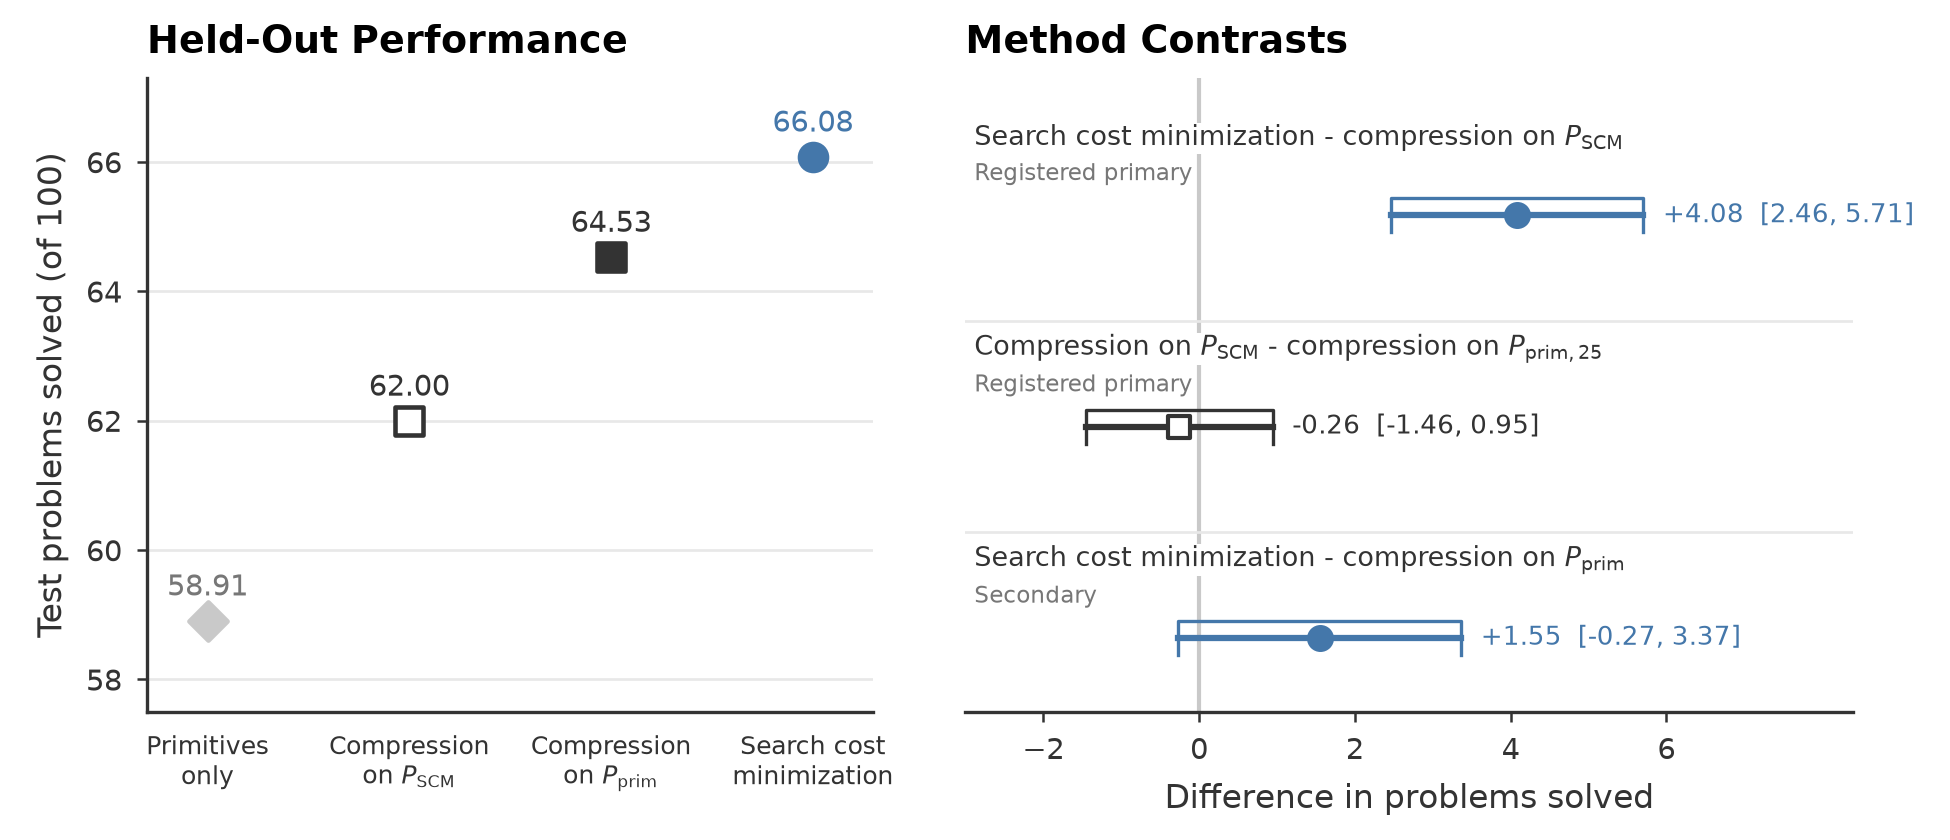
\includegraphics[width=\linewidth]{study_1_selection.png}
  \caption{Experiment I held-out results with ten abstractions. The left graph shows
  means, while the right graph shows paired differences with 95\% Student's $t$
  intervals for 30 seeds. Both procedures use the same problems of
  $T_{\mathrm{SCM}}$. Search cost minimization includes failures;
  compression on $P_{\mathrm{SCM}}$ omits unsolved targets. The
  second contrast compares compression on $P_{\mathrm{SCM}}$ with
  compression on $P_{\mathrm{prim,25}}$.}
  \label{fig:study1-selection}
\end{figure}
Selection itself costs search, and later search savings must recover that
cost for a more expensive selection method to be useful. Search cost
minimization has a higher initial search cost than compression because it
performs one bounded search for each trial library and scores all 25 problems
of $T_{\mathrm{SCM}}$ from its output record. We therefore estimate a
break-even point: the number of future problems whose search savings recover
that higher initial cost. The median break-even
point was several thousand future problems, and some seed-condition cases
never reached it. Figure~\ref{fig:study1-cost} gives the exact selection
costs, median break-even points, and case counts.
\FloatBarrier
\begin{figure}[!htbp]
  \centering
  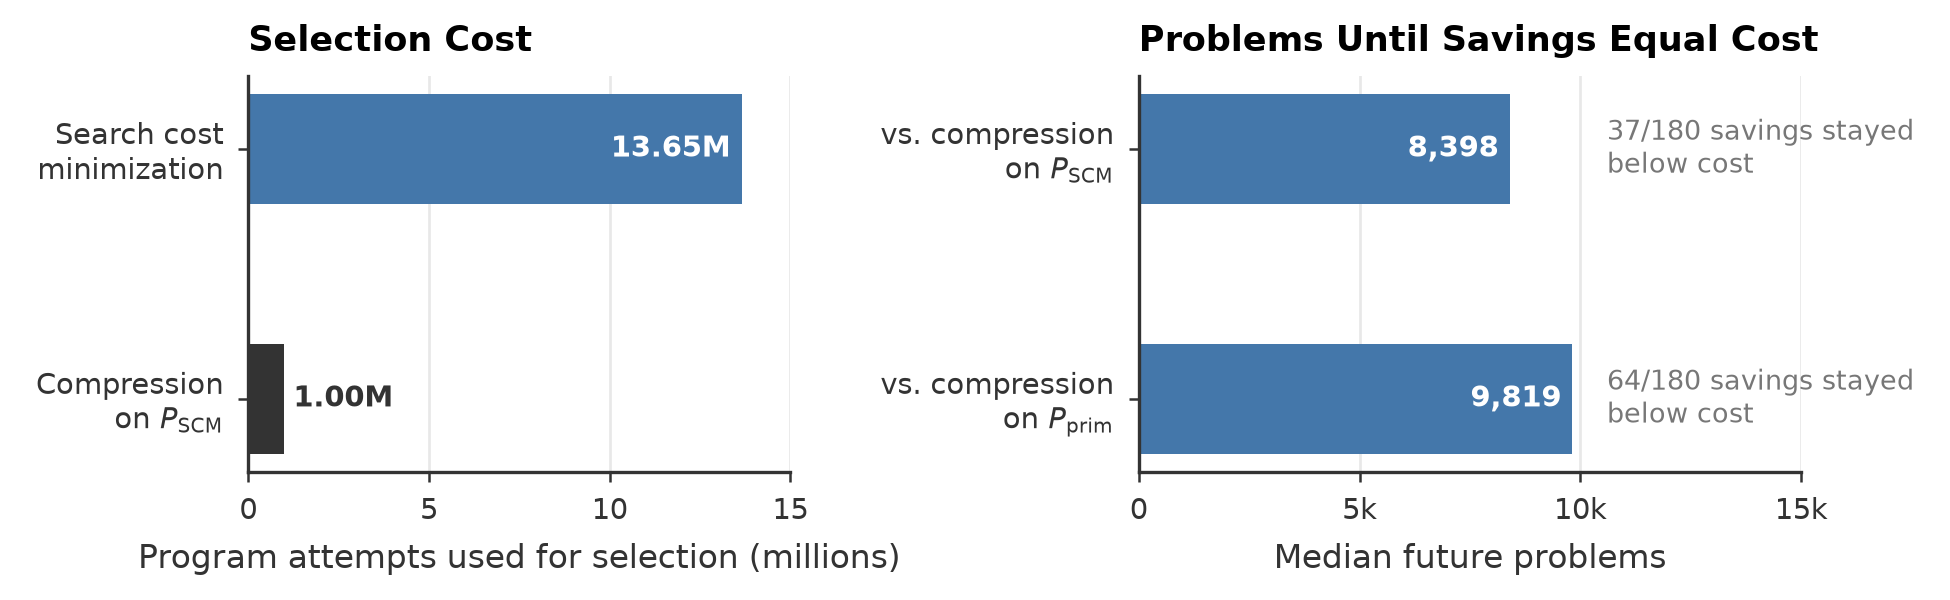
\includegraphics[width=\linewidth]{study_1_cost.png}
  \caption{Selection cost and break-even estimates. Gray labels mark cases
  with no break-even point. Counts are program attempts
  only; they omit the acquisition of
  $P_{\mathrm{prim}}$, wall-clock time, and segmentation.}
  \label{fig:study1-cost}
\end{figure}
\FloatBarrier
We expected compression to benefit from similar motifs in
$T_{\mathrm{prim}}$ and $T_{\mathrm{test}}$, and the
means followed that direction: search cost minimization minus compression on
$P_{\mathrm{prim}}$ decreased as problem-set similarity increased, from
2.7 problems for different sets to 1.5 for moderately similar sets and 0.5
for similar sets (left graph in Figure~\ref{fig:study1-secondary}). The
different-set interval excluded zero, showing search cost minimization's
advantage in that group. The formal tests follow the two similarity
measures. By assigned shift, moving from $\alpha=0$ to $\alpha=1$ changed
search cost minimization minus compression on $P_{\mathrm{prim}}$ by 2.10
problems (95\% CI [$-0.12$, 4.32]) and search cost minimization minus
compression on $P_{\mathrm{SCM}}$ by 1.70 (95\% CI [$-0.56$, 3.96]). By
realized similarity, the seed-controlled slope against $\rho$ was $-1.44$
for the $P_{\mathrm{prim}}$ difference (95\% CI [$-3.18$, 0.30]) and
$-0.36$ for the $P_{\mathrm{SCM}}$ difference (95\% CI [$-2.43$, 1.71]).
These intervals all included zero, so the formal tests did not establish
the hypothesized effect.
The two objectives could also overlap: abstractions chosen for search cost
might compress solutions as a side effect. We tested this by applying each
library post hoc to one fixed solution set, the solutions acquired for the
25-problem primitive-only subset (right graph in
Figure~\ref{fig:study1-secondary}). Direct compression on those problems
removed 25.78\% of operations; search cost minimization
scoring the same 25 primitive-only problems removed 12.32\%; search cost
minimization scoring the 25 problems of $T_{\mathrm{SCM}}$ removed
9.79\%. Search cost minimization shortened solutions indirectly, but direct
compression removed more.
\FloatBarrier
\begin{figure}[!htbp]
  \centering
  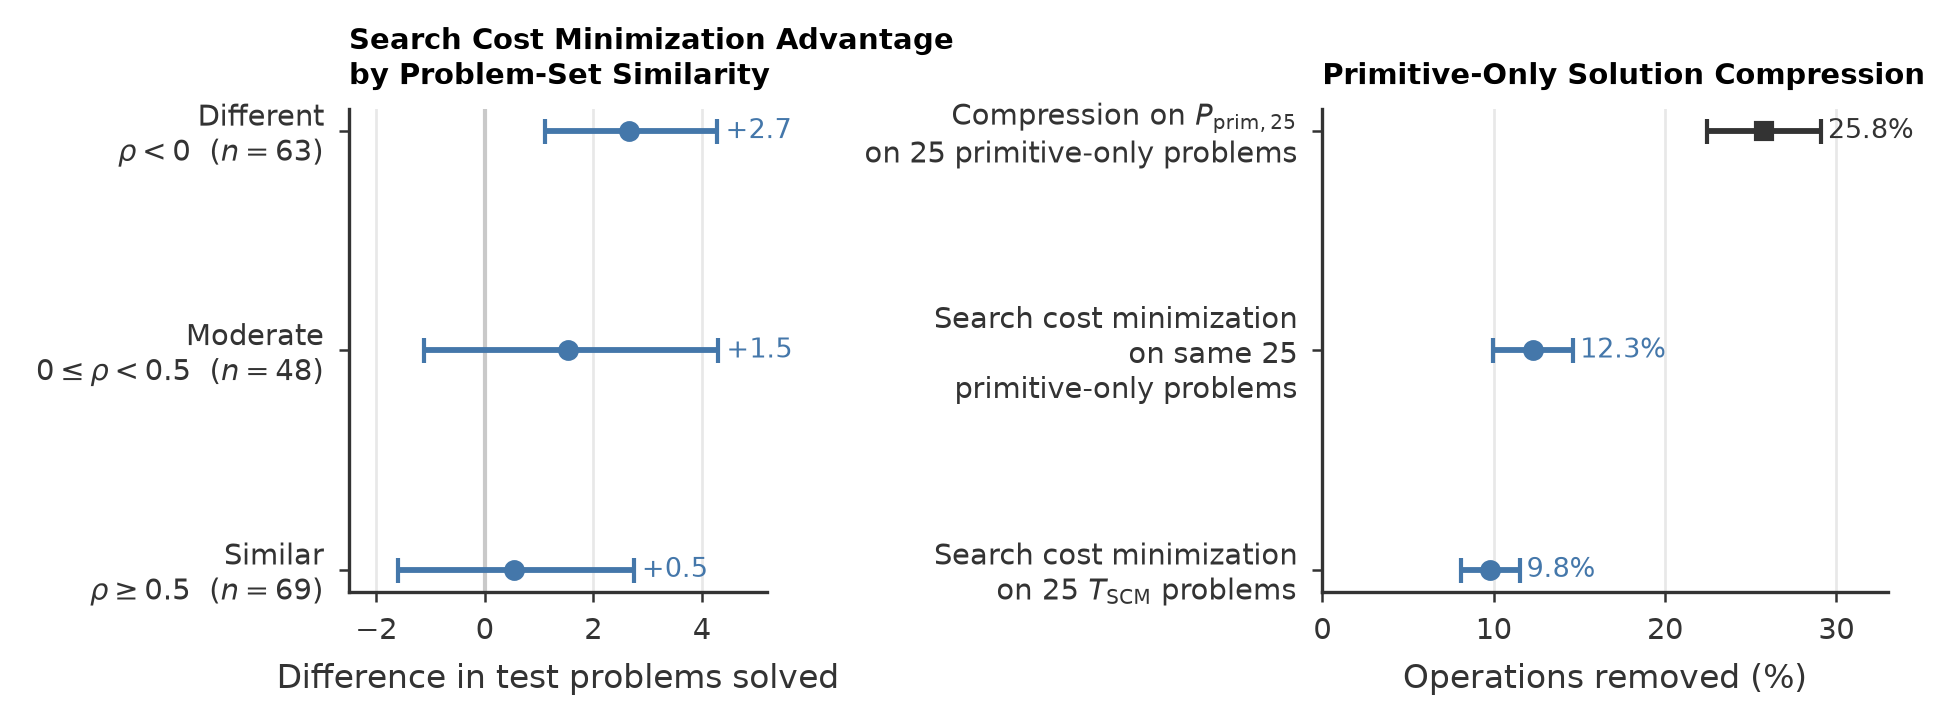
\includegraphics[width=\linewidth]{study_1_secondary.png}
  \caption{Problem-set similarity and indirect compression. Left: search cost
  minimization minus compression on $P_{\mathrm{prim}}$ at three
  problem-set similarity levels. Right: post hoc operations removed from the
  same primitive-only solutions. Intervals are 95\% seed-cluster and seed
  bootstrap, respectively; problem-set similarity bands were not registered.}
  \label{fig:study1-secondary}
\end{figure}
\subsection{Experiment II: Library Size}

Held-out performance did not change steadily as library
size increased
(Figure~\ref{fig:capacity-budget}). From ten to twenty abstractions,
compression on $P_{\mathrm{prim}}$ lost 12.35 problems
(simultaneous 95\% CI [$-13.89$, $-10.81$]), and search cost minimization
lost 12.11 (simultaneous 95\% CI [$-13.20$, $-11.02$]). At twenty
abstractions, both libraries solved fewer problems than the primitive
library. Between procedures, search cost minimization exceeded compression
on $P_{\mathrm{SCM}}$ by 5.13 problems (simultaneous 95\% CI [3.45,
6.80]) and compression on $P_{\mathrm{prim}}$ by 1.73 (simultaneous 95\%
CI [$-0.17$, 3.63]), and its advantage over compression on
$P_{\mathrm{SCM}}$ increased by 1.85 from ten to twenty (simultaneous
95\% CI [$-0.03$, 3.73]). Thus, library size had a larger effect on
absolute performance than on method differences.

At $B=30{,}000$, the descriptive means were highest at $K=11$: 66.32 for
compression on $P_{\mathrm{prim}}$ and 67.85 for search cost
minimization. From $K=1$ to $K=2$, compression on $P_{\mathrm{prim}}$
lost 8.08 problems, and search cost minimization lost 6.14, a drop that
Experiment III investigates. For compression on $P_{\mathrm{prim}}$,
operations removed from primitive-only solutions increased from 24.14\% at
$K=11$ to 27.21\% at $K=20$, while held-out performance decreased over the
same range, so more compression did not ensure better bounded search.
\subsection{Experiment III: Search Budget}

\begin{figure}[!t]
  \centering
  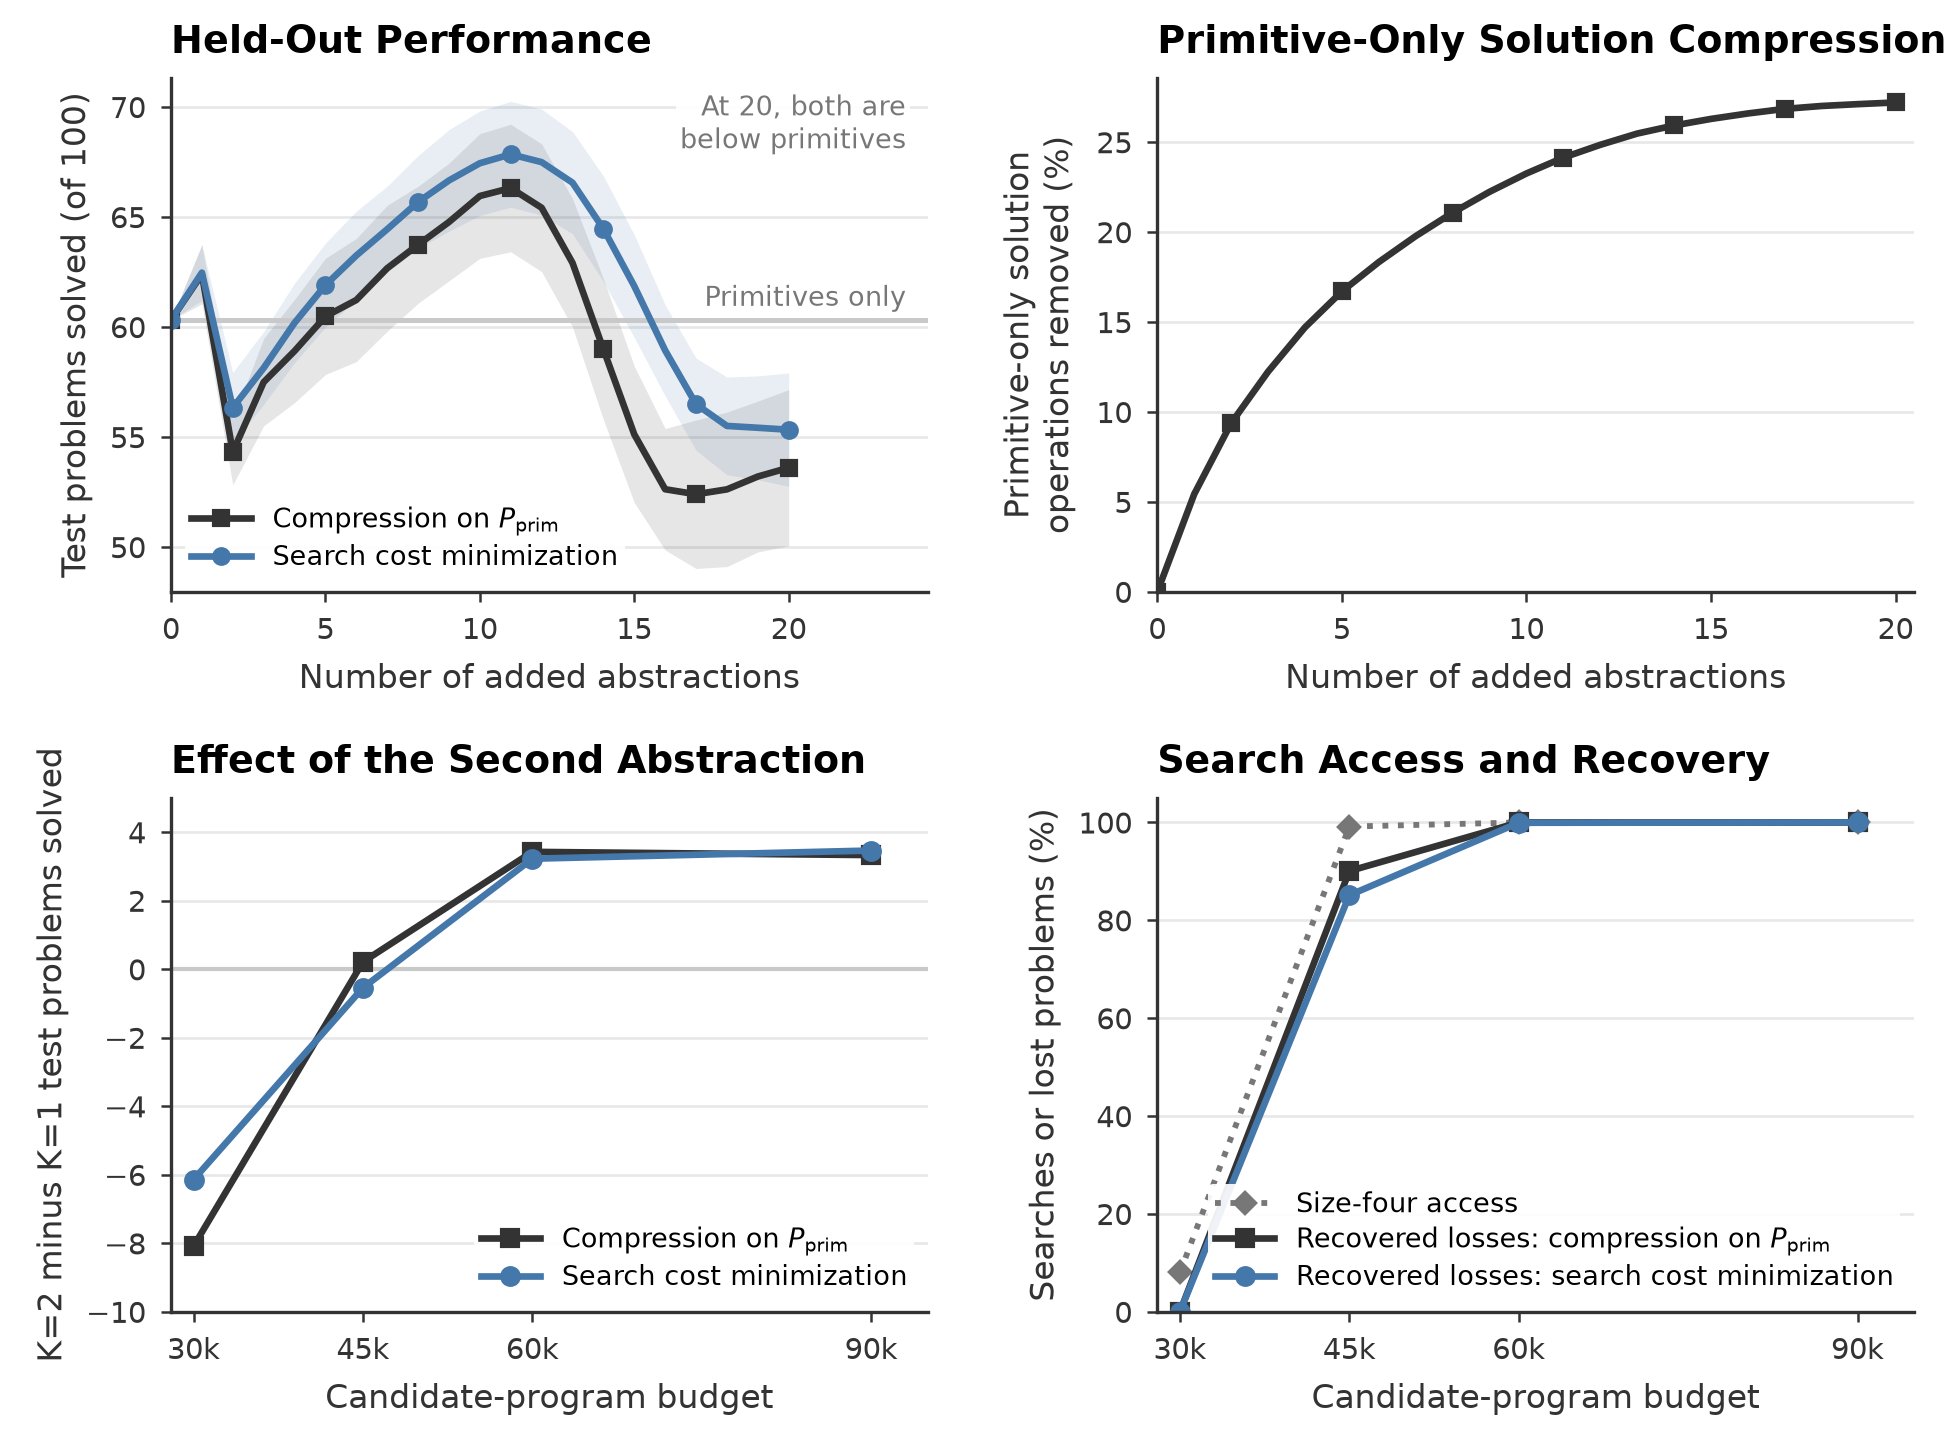
\includegraphics[width=\linewidth]{study_2_3_capacity_budget.png}
  \caption{Experiments II and III. The top row shows held-out performance and
  the compression of primitive-only solutions across library sizes. The
  held-out bands are simultaneous 95\% intervals. The compression graph is
  post hoc. At $K=0$, the library has only primitives. The bottom row shows
  the fixed-library budget test, the share of enumerations that reached
  size-four programs, and the descriptive recovery of lost problems.}
  \label{fig:capacity-budget}
\end{figure}
An increased budget
reversed the one-to-two decrease for the fixed libraries
(Figure~\ref{fig:capacity-budget}). As the budget increased from 30,000 to
90,000 program attempts, the second-abstraction effect increased by 11.42
solved problems for compression on $P_{\mathrm{prim}}$
(simultaneous 95\% CI [10.17, 12.66]) and by 9.61 problems for search cost
minimization (simultaneous 95\% CI [8.52, 10.69]). At
$B=90{,}000$, the effects were 3.33 for compression on
$P_{\mathrm{prim}}$ and 3.47 for search cost minimization. All
seed-level interactions were positive. The share of enumerations that
reached size-four programs shows whether the budget let the solver reach the
larger programs where an abstraction can help: with two abstractions, it
increased from 8.1\% at 30,000 attempts to 99.2\% at 45,000 and 100\% at
60,000.
By $B=90{,}000$, the solver recovered all test instances that the
two-abstraction library lost relative to the one-abstraction library at
$B=30{,}000$. Only the budget changed, so the 30,000-attempt budget caused
the one-to-two decrease for these fixed libraries. This result does not set a
sufficient budget for other libraries, solvers, or benchmarks.

\FloatBarrier

\section{Discussion}

This paper's main conclusion is that an abstraction's value depends on the
context in which the solver uses it: the problems and scoring rule used for
selection, the library's contents, future problems, the solver, the search
budget, the selection cost, and expected reuse. The conclusion matters
because many systems select abstractions by compressing known solution
programs, and prior work described the tradeoff a compression score can
hide: stored items shorten solutions while enlarging the search
\citep{iba1989macro}. Our experiments measure that tradeoff directly, and
the sharpest case is Experiment II, where more compression came with worse
bounded search.

Experiment I compares the complete selection procedures. Search cost
minimization minimized capped search cost for all 25 problems of
$T_{\mathrm{SCM}}$, including failures, whereas compression on
$P_{\mathrm{SCM}}$ minimized operations in acquired solutions for
the same problems but omitted unsolved ones. With ten abstractions, search
cost minimization solved 4.08 more held-out test problems than compression on
$P_{\mathrm{SCM}}$, which supports the hypothesis that it selects
more useful abstractions when both procedures use the same selection
problems. Scoring libraries in use also charges for the programs each
abstraction adds, so search cost minimization can favor lower net search
cost. However, the
4.08-problem difference depends in part on which problems of
$T_{\mathrm{SCM}}$ produced solutions, so it does not isolate
scoring-rule effects. Search cost minimization's 1.55-problem advantage over
compression on $P_{\mathrm{prim}}$ remained uncertain; compression on
$P_{\mathrm{prim}}$ scored four times as many problems, and solutions
from more problems could explain the smaller difference, which this
experiment did not test.

The match between selection and future problems could change abstraction
value, so we hypothesized that compression on primitive-only
solutions would become more competitive as the motif frequencies of
$T_{\mathrm{prim}}$ and $T_{\mathrm{test}}$ became more
similar. The means followed this pattern: search cost minimization's
advantage over compression on $P_{\mathrm{prim}}$ fell from 2.7
problems for different sets to 0.5 for similar sets. However, the formal
intervals included zero, so the formal comparisons remain inconclusive. This
direction is plausible because compression rewards stored grids that replace
subtrees in primitive-only solutions, and recurring motifs can let those
grids shorten test solutions. Our problem-set similarity measure, though,
ranks only motif counts and omits operation context, exact grid reuse,
program position, and search order. Similar motif counts do not ensure
similar search value.

Experiment II showed that abstraction value depends on library size. At 30,000
attempts, observed mean performance was highest at 11
abstractions and fell below the primitive library at 20. Compression on
$P_{\mathrm{prim}}$ removed more operations from primitive-only
solutions as its library grew
from 11 to 20 abstractions, even as held-out performance decreased. Each
abstraction is a size-zero item whose combinations with operations and other
library items create new low-operation programs. The solver examines them first, so
they can use the budget before it reaches a larger program where the
abstraction helps. A new
item also changes when the solver reaches programs that use earlier items.
Thus, operation removal measures a shortcut within known solutions but does not
measure the search required to reach those solutions.

Search budget can determine whether this added search prevents a solution or
only delays it. Experiment III changed only the budget for fixed one- and
two-abstraction libraries, and the larger budget reversed the one-to-two loss
for both procedures, supporting the hypothesis that a larger budget reverses
the loss for those libraries. The size-four diagnostic gives descriptive
support for the search-cutoff explanation.

Selection cost creates a separate tradeoff because future savings must recover
the initial cost. Search cost minimization required a bounded search for every
trial library, and among cases with a break-even point, the median required
thousands of future problems. Some experimental cases never reached that
point. Compression starts cheaper when representative solutions already
exist.

\section{Limitations and Future Work}

Experimental controls make changes in bounded search easier to identify, but
they limit where the results can apply. This study tests one synthetic,
target-only grid benchmark. Every abstraction is a stored output grid with size
zero, while the primitives, operations, program-size limit, and target generator
stay fixed.
Learned functions and parameterized abstractions can apply across inputs and
produce different search costs. Future work should repeat these experiments on
input--output synthesis tasks and in other domains.
A direct comparison of stored grids and learned functions should hold the
solver and budget fixed.

The search-cutoff explanation also depends on the solver. This solver performs
deterministic bottom-up enumeration and orders programs by operation count,
so library order and duplicate removal affect when it reaches a target. A
guided solver could prune low-value combinations or reach useful larger
programs sooner. Future studies should compare deterministic enumeration with
guided search and test other costs for abstraction use. A joint sweep can test
whether library size and test performance have the same relation under other
budgets.

Candidate discovery also limits how broadly the results apply. All procedures
select from the same 50 candidates derived from
$T_{\mathrm{prim}}$, so search cost minimization cannot select an
abstraction outside this set. The candidate set favors grids that support at
least two targets of $T_{\mathrm{prim}}$ and first appear in
programs with one to four operations. Experiment II evaluates prefixes of one
greedy sequence rather than optimizing each library size. Future work should
vary candidate-set construction and compare greedy selection with joint
selection of library items and their order. A selection objective could also
charge for the new programs that each candidate adds.

The primary Experiment I comparison evaluates complete procedures, so it does
not isolate scoring-rule effects. Search cost minimization scored all 25
problems of $T_{\mathrm{SCM}}$ and their failures, whereas
compression on $P_{\mathrm{SCM}}$ scored only acquired solutions,
so the 4.08-problem gap includes differences in what each procedure scores
and whether it includes unsolved problems. Compression on
$P_{\mathrm{prim}}$ used solutions acquired from 100 primitive-only
problems and therefore used more scoring problems from a different set. To
isolate scoring-rule effects, a comparison should use fixed target-solution
pairs: search cost minimization would score the targets, compression would
score their solutions, and solution acquisition would be fixed before data
collection. The similarity measure has a separate limit: it requires hidden
motif counts from completed test data, so it cannot guide deployment. Future work should define the measure before data collection,
vary compositional structure directly, and use more independent seeds to improve
precision.

Several findings need independent confirmation. The observed performance peak
near 11 abstractions and the one-to-two decrease were descriptive.
Experiment III reused the Experiment II seeds and fixed one- and
two-abstraction libraries, so its budget effect applies only to those libraries
and is not an independent replication. An independent test should use new seeds
and libraries. A broader sweep can identify the budgets needed to reach
programs that use added abstractions.

Finally, the break-even analysis counts only program attempts, omitting
wall-clock time, memory use, and compression segmentation. The comparison
with compression on $P_{\mathrm{prim}}$ treats the prior
acquisition of those solutions as
sunk. The calculation assumes constant mean savings across future problems.
Future work should measure end-to-end acquisition, selection, and evaluation
costs for expected workloads under distribution change.

\section{Conclusion}

The introduction asked how a solver should select abstractions from its
experience if its goal is maximum problem-solving performance on an unseen
test problem set. With ten abstractions, search cost minimization
outperformed compression on $P_{\mathrm{SCM}}$ by solving 4.08 more test
problems out of 100, in a comparison of complete procedures. Its advantage
over compression on $P_{\mathrm{prim}}$ remained uncertain, and mean
performance differences across problem-set similarity levels followed the
problem-set similarity hypothesis while their formal intervals included
zero.

The deeper lesson is that the same abstractions can help or hurt depending
on the library around them and the search the solver is allowed. At 30,000
attempts, both procedures improved on primitive-only search with ten
abstractions, and mean performance peaked near 11 before falling below
primitives alone at 20. Compression on $P_{\mathrm{prim}}$ removed more
operations from primitive-only solutions over this range while held-out
performance decreased, so solution compression alone was an incomplete
measure of bounded-search value. Each added item made more low-operation
programs available, which the solver examined before later programs where
the item could help, and for the fixed one- and two-abstraction libraries,
search budget determined whether the solver reached those later programs:
increasing only the budget reversed the one-to-two loss, supporting the
search-cutoff explanation for those libraries.

An abstraction's value must also cover how the abstraction was found. Search
cost minimization's added selection work often required thousands of future
problems to recover and did not recover in some cells. One factor stayed
fixed throughout: the search process. Every result here comes from one
deterministic solver, and a different search process could change the value
of every library we measured. A practical system
should therefore evaluate its complete library with its intended solver,
budget, workload, and expected reuse. A useful abstraction must save more
search than its selection and added programs cost on that workload.

\section*{Code and Data Availability}

Code, generated data, and reproduction instructions are available in a public
repository.
\par\smallskip
\noindent
\href{https://github.com/cucupac/program-synthesis}{%
\mbox{\texttt{github.com/cucupac/program-synthesis}}}.

\bibliography{references_rlj2026}
\bibliographystyle{rlj}

\end{document}
